%!TEX root = ../thesis.tex
%*******************************************************************************
%*********************************** Nineth Chapter *****************************
%*******************************************************************************

\chapter{Data collected from Ultrasound Doppler, PPG and LDF}  %Title of the First Chapter

\ifpdf
\graphicspath{{Chapter9/Figs/Raster/}{Chapter9/Figs/PDF/}{Chapter9/Figs/}}
\else
\graphicspath{{Chapter9/Figs/Vector/}{Chapter9/Figs/}}
\fi

The whole experiment also included the measurement of physiological changes using another set of instruments. As detailed in chapter \ref{chapter procedure}, devices such as an Electrocardiogram, Doppler Ultrasound, Laser Doppler Flowmetry and PPG in the red spectrum were used to collect data related to changes in flow and volume in different sections of the forearm and fingers. 

The ECG was used to record the electrical signals of the heart and its synchronicity with the other signals. The time difference between the ECG's R-wave and the systolic peak of the other signals produces the pulse transit time (PTT) which is useful to determine other physiological parameters such as blood pressure~\cite{liu2017cuffless}. The Doppler ultrasound which was located close to the radial artery in the wrist was used to estimate the speed of blood flow at this point. The PPG placed in the index finger provides information about the changes of volume in the vascular bed around the fingers area. Finally, the Laser Doppler Flowmetry attached to the mid-section of the forearm measures changes of RBC in the vascular bed around the arm. 

%%********************************** % Section 9.1 ******************************************
\section{Measurements from the ECG device}
\label{section comparison 1}
The ECG signals collected provide details of the electrical activity of the heart during the whole study. Hence, extreme changes in the heart rate or shape were not registered through the test unless a bad connection occurred. The data gathered also worked as a clock reference during the data processing. Figure \ref{fig:ECG} shows the typical ECG for one of the participants.

\begin{figure}[!htbp]
	\centering
	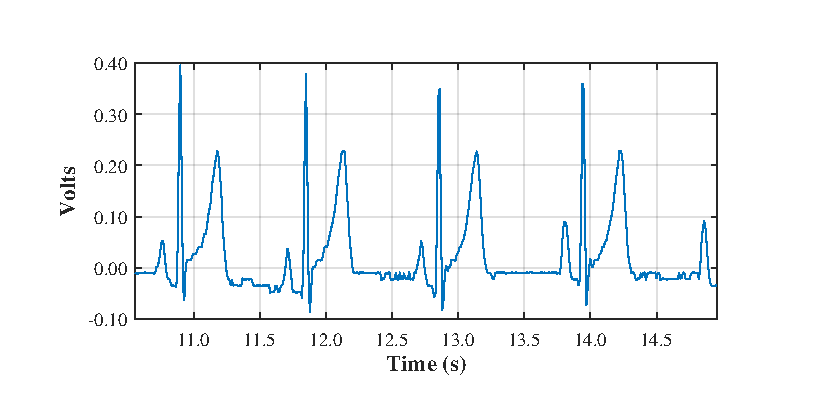
\includegraphics{figure19}    
	\caption[ECG measurement acquired by the system]{Measurement from one of the participants. Clearly, it can be identified the points P, Q, R, S and T. This signal did not change during the whole experiment.}
	\label{fig:ECG}
\end{figure} 

All the waveforms detected were typical and provided enough information about the characteristic peaks in an ECG waveform. The points P, Q, R, S and T were visible in all the signals. Nonetheless, Participant 1 showed an elevated T-wave which is presumably due to his athletic vocation. According to him, he had a ventricular hypertrophy meaning that one of his ventricles was enlarged.  

%%********************************** % Section 8.3 ******************************************
\rvmynote{This part was added from chapter 8. I need to check the flow form the introduction an the conclusion of this chapter}
\section{Blood flow calculation from arterial pulses signal}
\label{section apa flow arterial pulses}
So far the blood flow has been analysed from occlusive methods using the techniques described in section \ref{section literature VOP}. However, these procedures require mechanical occlusion to produce an increase in volume within the forearm being measured. Nevertheless, sometimes this can be uncomfortable, especially when the applied pressure is above the systolic value or when the person just can not tolerate restriction of blood flow.

For these cases, analysing the waveform also provides information about the blood flow. The rush of blood into the vessel creates a small increase in volume within the limit of the potential electrodes which can be translated into a quantifiable blood flow. Having a device sensitive enough to detect these changes is crucial to provide an accurate estimation of the blood speed. As described in section \ref{section iPG waveforms}, the waveform contained within the basal impedance was amplified by the device, achieving great detail.

In fact, different studies have demonstrated that it is possible to calculate blood flow from the analysis of the APA waveform \cite{corciova2011peripheral, costeloe1980continuous, brown1975impedance}. In this case, the change of impedance used to perform this calculation occurs between the foot of the wave and the systolic peak. This $\Delta Z$ is used to calculate blood flow by also applying Nyboer's equation \ref{eq:nyober dV}.

\begin{figure}[!htbp]
	\centering
	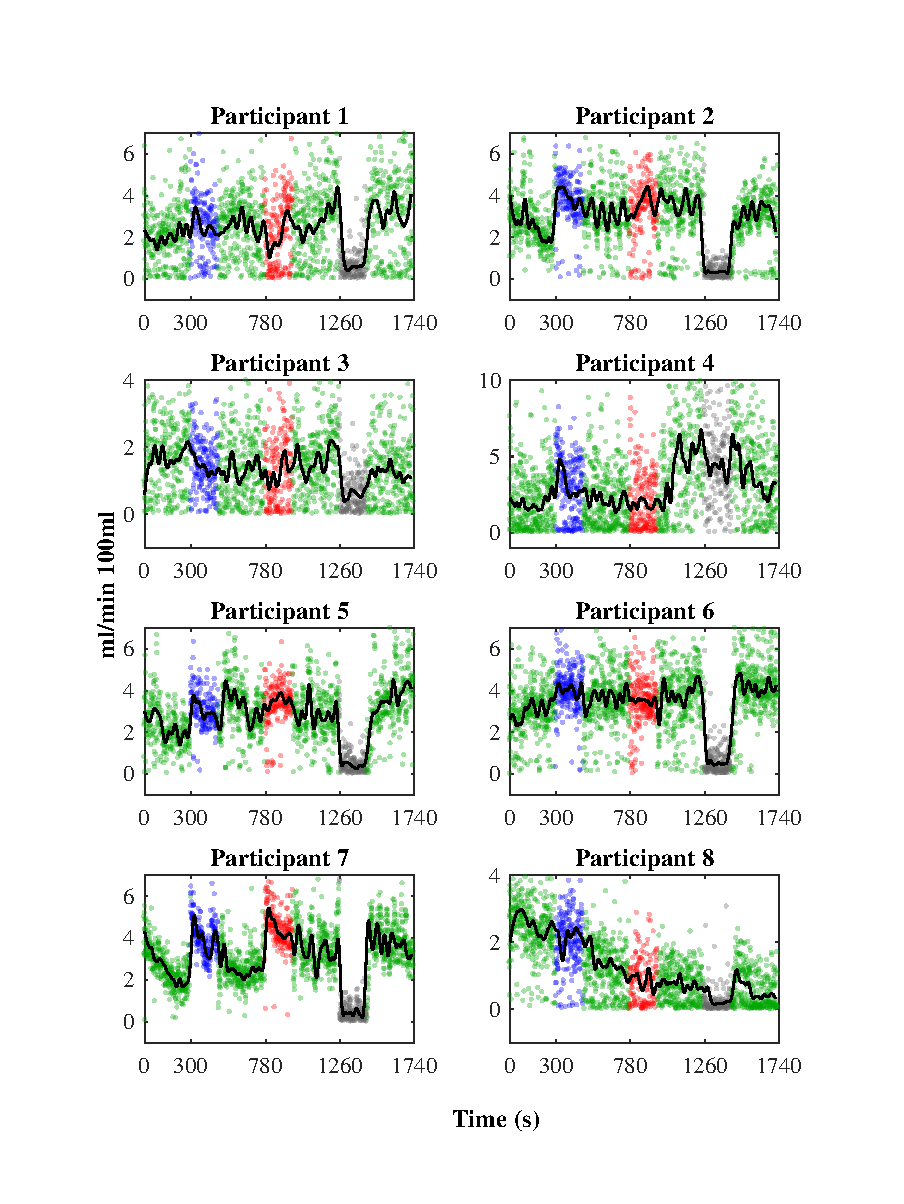
\includegraphics[width=0.85\textwidth,trim={1.5cm 0.5cm 1.5cm 1.5cm},clip]{figure_apa_8}
	\caption[Blood flow calculated from impedance plethysmography waveform at the time of the whole expetiment]{Blood flow calculated for all the participants during the experiment. Each dot represents the peak value of the waveform that has been converted into flow (\si{\bfv}). The green dotted area represent the baselines measurements (regions 1,3,5 and 7). The region 2 (venous occlusion) is represented by the blue dots, arterial occlusions (region 4) are in red and total occlusions (region 6) are in grey.}
	\label{fig:blood_flow_plethysmography}
\end{figure}

Figure \ref{fig:blood_flow_plethysmography} shows the blood flow derived from the amplitude of the systolic peak throughout the whole experimental session. Green dots show blood flow measurements during baseline readings (regions 1, 3, 5 and 6). The other colours indicate the venous occlusion in blue, partial arterial occlusion in red and total obstruction in grey. The dark line drawn above the signals corresponds to the smoothing of each measurement event using \textit{robust loess} method of the \textit{smooth} command in Matlab. Overseeing the amplitude transition in each region will help explain how the flow changes with each occlusive event. The value of the calculated blood flow shown in the same figure does not include the negative sign which represents the direction of flow relative to the potential electrodes.

As portrayed in the same figure, between each transition, in the middle of baseline and occlusion, some participants described clearly marked shifts in the calculated flow. In most participants, when venous occlusion occurred, the change between baseline and venous occlusion created a blood surge followed by a tendency for the flow to stabilise. It is worth noting that the increment of blood flow in participant 2 occurred before the venous occlusion. The reason for this is that the obstruction probably started before \SI{300}{\second} and the pressure applied to the arm was rather slow. There are other cases where the flow change occurred so fast that an entirely blank space can be seen connecting both events, as in participants 5 and 7. This situation, as opposed to participant 2, was more likely due to the cuff being inflated faster which did not allow a gradual but instead sudden change in flow. However, also, it could be related to a physiological response of the body like vasodilation response, where one reacts faster than others. Finally, participant 8 is an exception to this rule. This participant experienced a decrease in the calculated flow, followed by a stabilisation. A flow surge is not identifiable in this partaker.

Between venous occlusion and return to baseline in region 3, the cuff was rapidly deflated to restore blood flow to a normal condition. However, from the calculated data it can be seen that there are no extreme changes in blood flow between these two sections as soon as the blockage was released. As noted, in most participants except partakers 5 and 7, there are little changes between these two sections indicating that there is a slight change in blood flow. This action can be linked to a hyperaemic effect where as soon as the pressure of the cuff is released, the blood contained within the vessels of the forearm runs out to the upper part of the arm. After that, the blood flow tended to stabilise towards an average value.

Similarly, as between regions 1 and 2, the change between baseline (region 3) and partial arterial occlusion (region 4 - red colour) generated alterations in the calculated blood flow. Some participants, like partakers 6 and 7 showed a rapid increase in blood flow after the occlusion followed by settling in the blood velocity, where the latter is more notorious. Others like participants 1, 2, 3 and 5 showed a Gaussian bell-shaped flow during the occlusion. It is evident that their flow did not set in a mean value. The only ones that enacted different behaviour were participants 4 and 8, where not much change of blood is evident. However, it is notorious the continuous change of amplitude in participant 8 at this point which is contrary to the rest of participants.

The change between partial arterial occlusion (red section) and baseline had a similar effect as the one described for the release of pressure of venous blockage. Most of the participants showed a decrease in their blood flow, right after the cuff's pressure was released, possibly caused by a hyperaemic effect. At this point, one can note that participant 4 started to show random blood flow readings.

Total occlusion (grey dots) had an expected response in almost all the study members. When the blood flow was completely stopped, it was anticipated that its calculated value could tend to zero. In this case, the device was able to detect these changes. The only exception was participant 4 who again showed random results. At this point, it was to be expected that something wrong was happening with his measurements. Then, when the tourniquet was released, the blood flow returned in an exponential form and then set to an average value. In this case, the hyperaemic effect is more visible. It is worth noting that participant 8 showed a decline in blood flow measurements towards the midpoint of the test. This event agrees, with the partaker expressing not feeling very well at the end of the test. One can speculate it is a coincidence, or maybe the device was able to detect these physiological changes in him.

It seems evident that there is a blood surge when an occlusion in the blood circulation occurs from the impedance computation. Subsequently, the blood flow tends to stabilise at an average value. When the blockage is released, it seems that in some cases the flow tends to decrease and in others, there is no apparent change. The following sections will discuss the results of the change in median blood flow during each occlusive event.


%%********************************** % Section 8.3.1 ******************************************
\subsection{Blood flow change during venous occlusion}
\label{sectio results 3.1}
The following are the results of calculating the median blood flow between baseline in region 1, venous occlusion in region 2 and the return baseline after releasing the cuff's pressure in region 3. Once again, the result of the calculation is the absolute value, dropping the negative sign as this indicates the direction of the flow relative to the electrodes. Table \ref{tbl:blood_flow_iPG_venous} sums up the results obtained by flow measurement in the scale \si{\bfv}. The mean blood flow in region 1 was about \SI{2.283(0437)}{\bfv}. When the venous occlusion took place by inflating the cuff below diastolic value, the average blood flow calculated in region 2 was \SI{3.034(0938)}{\bfv}. It is easy to see that there was in increase of blood flow in approximately \SI{33}{\percent} during this part of the experiment. It seems that this increment in the blood flow could be due to a physiological response. It seems that there is a vasodilation process allowing extra blood to be retained in the venous circulation. However, study members 3 and 8 showed a decrease in their blood flow during this transition of about \SI{0.386(0011)}{\bfv}. The latter is not a surprise, as it was noted before, all his recordings started to go downwards from the beginning of the test. In the case of the participant 3, the obtained data seems not well distributed towards the mean. Therefore, there must be a significant number of outliers within its measurement making difficult extracting the real median blood flow. 

Clearly, there is a blood flow fall when the cuff's tension was released to return to the baseline signal. Indeed, six out of eight of the participants experienced a drop in their flow rate during this part of the experiment. The average blood flow for region 3 was approximately \SI{2.409(0885)}{\bfv}, which is equivalent to a \SI{5.5}{\percent} difference with the initial baseline at region 1. On the contrary, participants 1 and 5 did not experience this reduction of flow rate but a slight increase of less than \SI{0.09}{\bfv} or \SI{3.9}{\percent} increment when compared to the original reference signal.

\begin{table}[h]
	\caption{Mean blood flow calculated form the plethysmography wave for baseline, venous occlusion and return to baseline}
	\label{tbl:blood_flow_iPG_venous}
	\centering
	\begin{tabular}{l
			*{3}{S[table-format=1.3]@{\,\( \pm \)\,}S[table-format=1.3]} %Format for Z+-std
		}
		\toprule
		& \multicolumn{2}{c}{\textbf{Region 1}}
		& \multicolumn{2}{c}{\textbf{Region 2}}
		& \multicolumn{2}{c}{\textbf{Region 3}}  \\
		& \multicolumn{2}{c}{\small{\si{[\bfv]}}}
		& \multicolumn{2}{c}{\small{\si{[\bfv]}}}
		& \multicolumn{2}{c}{\small{\si{[\bfv]}}} \\\midrule
		Participant 1 & 2.046  & 1.772 & 2.688  & 1.638 & 2.710  & 1.481 \\
		Participant 2 & 2.516  & 1.185 & 3.766  & 1.161 & 3.119  & 1.252 \\
		Participant 3 & 1.794  & 1.282 & 1.416  & 0.796 & 1.325  & 1.260 \\
		Participant 4 & 1.811  & 2.032 & 3.296  & 2.010 & 1.748  & 1.959 \\
		Participant 5 & 2.033  & 1.082 & 3.024  & 0.947 & 3.110  & 1.277 \\
		Participant 6 & 3.054  & 1.289 & 4.019  & 1.146 & 3.566  & 1.330 \\
		Participant 7 & 2.555  & 0.930 & 3.993  & 0.924 & 2.483  & 0.827 \\
		Participant 8 & 2.461  & 0.874 & 2.068  & 0.901 & 1.207  & 0.729 \\
		\bottomrule
	\end{tabular}
\end{table}

%********************************** % Section 8.3.2 ******************************************
\subsection{Blood flow change during partial arterial occlusion}
\label{section apa 3.2}
The change of blood flow between the baseline (region 3) and partial arterial occlusion (region 4)  was not as evident as the response seen in the previous section, where most of the participants showed an increase in their calculated flow rate. Certainly, three out of eight participants reported an increase in their blood flow, whereas in the rest decreased.  In general, the average flow rate during baseline was \SI{2.408(0885)}{\bfv}. Later, during the partial arterial occlusion, the mean blood flow increased in just \SI{8.4}{\percent} to approximately \SI{2.612(1266)}{\bfv}. 

It is clear that the increase was not as notorious as the one seen all along venous occlusion. Indeed, participants 2, 5 and 7 showed an increment in their blood flow with a centre of \SI{0.889(0925)}{\bfv}, especially the latter had the greatest change of blood flow. Conversely, the rest of the participants exhibited a small decrease in their blood flow with an average of \SI{-0.208(0180)}{\bfv}.

When the upper arm pressure was released in the region 5, it was expected that most of the participants would show a slump in their flow rate. However, this was not the case. The average blood flow at this stage was \SI{2.973(1293)}{\bfv}, which is equivalent to an increment of \SI{23}{\percent} from the baseline region 3. More in detail, three study members depicted a drop in their rate (5, 7 and 8) with an average of \SI{-0.618(0431)}{\bfv}. The rest of the study members showed an increase in their data of about \SI{0.948(1263)}{\bfv}. Notwithstanding, as previously described in this region, participant 4 showed random values entirely outlying the median obtained. At this stage, it is not possible to draw a clear conclusion whether an arterial occlusion would produce an increase or decrease of blood flow from the impedance measurement.

\begin{table}[!htpb]
	\caption{Mean blood flow calculated form the plethysmography wave for baseline, partial arterial occlusion and return to baseline}
	\label{tbl:blood_flow_iPG_arterial}
	\centering
	\begin{tabular}{l
			*{3}{S[table-format=1.3]@{\,\( \pm \)\,}S[table-format=1.3]} %Format for Z+-std
		}
		\toprule
		& \multicolumn{2}{c}{\textbf{Region 3}}
		& \multicolumn{2}{c}{\textbf{Region 4}}
		& \multicolumn{2}{c}{\textbf{Region 5}}  \\
		& \multicolumn{2}{c}{\small{\si{[\bfv]}}}
		& \multicolumn{2}{c}{\small{\si{[\bfv]}}}
		& \multicolumn{2}{c}{\small{\si{[\bfv]}}} \\\midrule
		Participant 1 & 2.710  & 1.481 & 2.251  & 1.689 & 2.977  & 1.791 \\
		Participant 2 & 3.119  & 1.252 & 3.486  & 1.399 & 3.537  & 1.492 \\
		Participant 3 & 1.325  & 1.260 & 1.299  & 1.025 & 1.647  & 1.132 \\
		Participant 4 & 1.748  & 1.959 & 1.665  & 1.895 & 4.832  & 7.032 \\
		Participant 5 & 3.110  & 1.277 & 3.454  & 0.994 & 2.841  & 1.225 \\
		Participant 6 & 3.566  & 1.330 & 3.417  & 1.197 & 3.866  & 1.558 \\
		Participant 7 & 2.483  & 0.827 & 4.441  & 1.001 & 3.389  & 1.050 \\
		Participant 8 & 1.207  & 0.729 & 0.882  & 0.864 & 0.693  & 0.537 \\
		\bottomrule
	\end{tabular}
\end{table}

%********************************** % Section 8.3.3 ******************************************
\subsection{Blood flow change during total occlusion}
\label{section apa 3.3}
As previously explained in section \ref{section apa 2.3}, during total occlusion the APA amplitude was just a fraction of the baseline waveform.  Therefore, the $\Delta Z$ obtained to calculate the blood flow is a small number resulting in a low or null calculation. In this part of the analysis, the majority of the study members showed a decrease in blood circulation rate close to zero.  As is evident from table \ref{tbl:blood flow iPG total}, almost all participants registered a significant drop in their blood flow calculation when the blockage was applied in region 6. Once more, Participant 4 displayed a unique response during the occlusion which median blood flow did not go close to zero. Above all, the median calculated blood flow during the baseline region 5 was approximately \SI{2.972(1210)}{\bfv}. On the other hand, at the time of the brachial arterial constriction the flow rate reduced to about \SI{0.3953(1412)}{\bfv}. One would expect a completely zero at this point as clearly there is not blood flow passing through the forearm. However, this measurement could be considered the error of equipment measurement caused by noise picked up by the device. 

After the tourniquet had been withdrawn, the blood flow recovered exponentially, portraying a fast return to baseline accompanied by an overshot peak and followed by settling towards a midpoint, as shown in figure \ref{fig:blood_flow_plethysmography}. This kind of shape is typical of a hyperaemia where the return of blood flow produces this overshot response, because of the fast filling of the vessels. The mean blood flow in the region 7 was about \SI{2.892(1332)}{\bfv}, which is very close to the original baseline region 5. In fact, the calculated flow reduction was about \SI{2.6}{\percent}. Though, it can be seen that participant 8 had an expected drop in the flow rate before the blockage and then an increase in the rate. This event is fascinating as these changes occurred in a blood flow below \SI{1}{\bfv}, but the device was able to notice the swing of blood flow rate. At this stage, the sensitivity for calculation of small changes in blood flow needs improvement because it detected flow values in other participants when there was no plethysmography signal. However, it is quite remarkable to see that the instrument is capable of detecting changes in the trend.

\begin{table}[!htbp]
	\caption{Mean blood flow calculated form the plethysmography wave for baseline, total occlusion and return to normality}
	\label{tbl:blood flow iPG total}
	\centering
	\begin{tabular}{l
			*{3}{S[table-format=1.3]@{\,\( \pm \)\,}S[table-format=1.3]} %Format for Z+-std
		}
		\toprule
		& \multicolumn{2}{c}{\textbf{Region 5}}
		& \multicolumn{2}{c}{\textbf{Region 6}}
		& \multicolumn{2}{c}{\textbf{Region 7}}  \\
		& \multicolumn{2}{c}{\small{\si{[\bfv]}}}
		& \multicolumn{2}{c}{\small{\si{[\bfv]}}}
		& \multicolumn{2}{c}{\small{\si{[\bfv]}}} \\\midrule
		Participant 1 & 2.977  & 1.791 & 0.564  & 1.283 & 3.466  & 2.553 \\
		Participant 2 & 3.537  & 1.492 & 0.284  & 0.698 & 2.922  & 1.179 \\
		Participant 3 & 1.647  & 1.132 & 0.567  & 0.751 & 1.277  & 1.210 \\
		Participant 4 & 4.832  & 7.032 & 4.350  & 2.868 & 3.786  & 4.128 \\
		Participant 5 & 2.841  & 1.225 & 0.342  & 0.687 & 3.500  & 1.645 \\
		Participant 6 & 3.866  & 1.558 & 0.448  & 1.190 & 4.103  & 1.489 \\
		Participant 7 & 3.389  & 1.050 & 0.343  & 1.121 & 3.689  & 0.958 \\
		Participant 8 & 0.693  & 0.537 & 0.098  & 0.449 & 0.399  & 0.567 \\
		
		\bottomrule
	\end{tabular}
\end{table}


%%********************************** % Section 9.2 ******************************************
\section{Blood flow estimation from Doppler ultrasound instrument}
\label{section comparison 2}
As part of the experimental procedure, a Doppler ultrasound was used to estimate blood flow using the radial artery in the wrist as a reference. The raw data produced by the instrument came in volts which was later converted into more meaningful data using the equations \ref {eq:doppler} and \ref {eq:flow_l/min} which convert the information into units litres per minute (\si{\litre\per\minute}). As described in those equations, the angle was fixed to \SI{45}{\degree} using a laboratory support and a clamp. The cross-sectional area for calculating blood flow was the median value of~\cite {ashraf2010size}. The head of the ultrasound device was placed as close to the artery as described in the user manual of the instrument using a conductive gel as an interface between the skin and the device.

While taking the measurements, there was an electrical problem with the Doppler ultrasound instrument. Hence, it was not possible to collect data from participant 8. The data presented in figure \ref{fig:DU flow} and table \ref{tbl:DU flow} contains the results of the first seven study members.

\begin{figure}[!htb]
	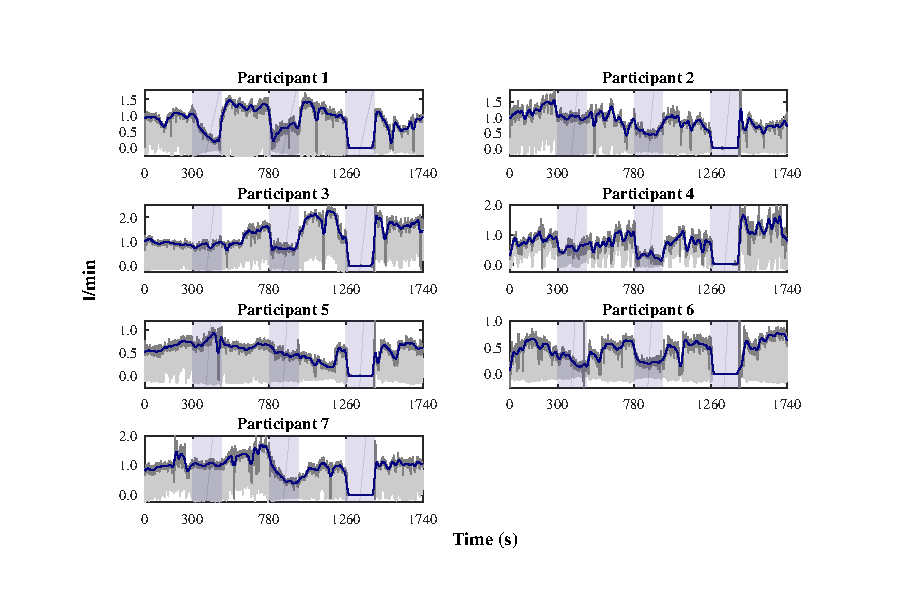
\includegraphics[width=\textwidth,keepaspectratio,trim={1cm 0cm 1.5cm 0cm},clip]{figure_cmp_2}    
	\caption[Blood flow calculated from Doppler ultrasond device all along the whole expetiment]{Blood flow calculated from the Doppler ultrasound measurements for all the participants during the experiment. The greyed out areas are the raw sign of the DU waveform. The dark blue lines represent the envelope calculated from the peak values. The blood flow was converted to the units (\si[per-mode=symbol]{\litre\per\minute}).}
	\label{fig:DU flow}
\end{figure}

%%********************************** % Section 9.2 ******************************************
\subsection{Blood flow estimation from Doppler Ultrasound instrument}
\label{section comparison 2.1}
Figure \ref{fig:DU flow} shows the peak values of the Doppler ultrasound converted into the arterial flow rate. The shaded areas represent the occlusive events during the study. The measurements depict the blood flow of the radial artery and the changes during each occlusive event. During venous occlusion, it was expected not to observe a significant change of the arterial flow rate as the brachial artery was not occluded above the diastolic pressure. On the other hand, a partial arterial occlusion between diastolic a systolic pressure restricts the inflow of affecting the blood flow towards the radial artery. Finally, at the moment of occluding the brachial artery above systolic pressure, it is expected to display null blood flow.

The qualitative analysis of the DU data shows that evidently, various participants showed an alteration in their calculated median arterial flow during venous occlusion in region 2. There were different types of responses, while some experience a rapid variation within the first few seconds, in others took some time to show a resting point. More in-depth, Participant 1 evidenced an exponential flow rate decrease during this part of the test. Further, participants 2 and 4 displayed a quick drop within the first seconds followed by a settling at a mid-point. Finally, the rest of the participants did not show a significant change in flow rate during this transition. Nevertheless, the quantified data showed in \ref{tbl:DU flow} illustrated that during the transition between baseline regions 1 and 2, five out of seven participants showed a drop in their median blood flow, being Participant 1 the most obvious with a drop of \SI{52.41}{\percent} of the blood speed. The other ones exhibited a slight decrease were partakers 2,3,4 and 6 where their blood flow was about \SI{25.80(1850)}{\percent}. On the other hand, study members 5 and 7 showed a slight increase of their calculated blood flow in \SI{10.16}{\percent} and \SI{6.25}{\percent} respectively. When the cuff's pressure was released, most of the participants showed a recovery in the detected blood flow. The only ones that showed a minimal drop were participants 2 and 5.

During partial arterial occlusion, unmistakable, the arterial blood flow changed in all the participants. In this case, it is clear that the narrowing of the brachial artery restricted the blood in the arm's arterial circulation altering the flow rate speed detected by the DU. As the figure shows, most of the participants showed a quick change of blood flow as soon as the constriction was applied, except participant 5. In general, the reduction of the blood flow in the radial artery was about \SI{48.79(1191)}{\percent}. As soon as the flow was restored, the majority of the participants experienced an increase in their blood flood caused by a rush of blood within the arterial circulation going through a quick rush of blood for few seconds. However, participant 5 described a different response which may have been caused by the misaligned of the sensor head.  

\begin{table}[!htb]
	\caption{Mean blood flow calculated form the Doppler Ultrasound waveform during all the regions of the experiment.}
	\label{tbl:DU flow}
	\centering \small
	\begin{tabular}{p{1.9cm}cccccccc}
		\toprule
		& \textbf{Region 1}
		& \textbf{Region 2}
		& \textbf{Region 3}
		& \textbf{Region 4}
		& \textbf{Region 5}
		& \textbf{Region 6}
		& \textbf{Region 7} \\
		& \textbf{[\si[per-mode=symbol]{\litre\per\minute}]}
		& \textbf{[\si[per-mode=symbol]{\litre\per\minute}]}
		& \textbf{[\si[per-mode=symbol]{\litre\per\minute}]}
		& \textbf{[\si[per-mode=symbol]{\litre\per\minute}]}
		& \textbf{[\si[per-mode=symbol]{\litre\per\minute}]}
		& \textbf{[\si[per-mode=symbol]{\litre\per\minute}]}
		& \textbf{[\si[per-mode=symbol]{\litre\per\minute}]} \\\midrule	
		Participant 1 & 0.954 & 0.430 & 1.285 & 0.618 & 1.049 & 0.003 & 0.719 \\
		Participant 2 & 1.211 & 1.014 & 0.967 & 0.546 & 0.843 & 0.002 & 0.712 \\  
		Participant 3 & 0.928 & 0.860 & 1.307 & 0.716 & 1.940 & 0.002 & 1.675 \\  
		Participant 4 & 0.826 & 0.581 & 0.764 & 0.297 & 0.754 & 0.002 & 1.245 \\  
		Participant 5 & 0.643 & 0.708 & 0.655 & 0.483 & 0.348 & 0.003 & 0.606 \\  
		Participant 6 & 0.495 & 0.248 & 0.499 & 0.230 & 0.542 & 0.002 & 0.641 \\  
		Participant 7 & 0.962 & 1.022 & 1.320 & 0.535 & 0.876 & 0.002 & 1.040 \\  	 
		\bottomrule
	\end{tabular}
\end{table}

Finally, all along with total occlusion, the tourniquet effect can be noticed in the composition of the signal with a sharp drop as soon as the occlusion took place. As expected, no arterial flow was recorded, the minimum values registered might represent artefacts in the signals. After releasing the tourniquet, all the participants experienced an increase in their flow rate to values of normality. 

%%********************************** % Section 9.3 ******************************************
\section{Measurements from Laser Doppler Flowmetry}
\label{section comparison LDF}
The LDF device provided raw data in Volts which was converted into BPU units. This conversion was possible by applying equation \ref{eq:BPU} to the data collected. As explained in section \ref{section:ldf}, the result produced is in an arbitrary unit which represents blood cell movement under the micro-circulatory bed of the skin. This unit known as BPU is the product of the mean number of moving blood cells in the small volume under the probe and the average velocity of moving red blood cells in the forearm. Converting the raw data to BPU unit was possible due to the equation \ref{eq:BPU}.

Figure \ref{fig:LDF flow} displays the peaks of the LDF waveform signal in BPU. The grey points are the raw data of the measurements. The purple line in the figure represents the smoothed signal averaged per heartbeat. The boxed areas describe the data portions where the occlusions took place. That plot shows that evidently the movement of the blood cells is affected when an occlusion occurs. Indeed, there is a diminution of the magnitude of the signal during each flow restriction. During the experiment, the LDF signal was very susceptible to noises; this explains the massive peaks seen during some the measurements. Especially participants 1 and 3 depicted a significant number of high peaks. From the qualitative point of view, it is explicit that heavily impacted some parts of the data, such as in participants 1 and 4.

\begin{figure}[!htb]
	\centering
	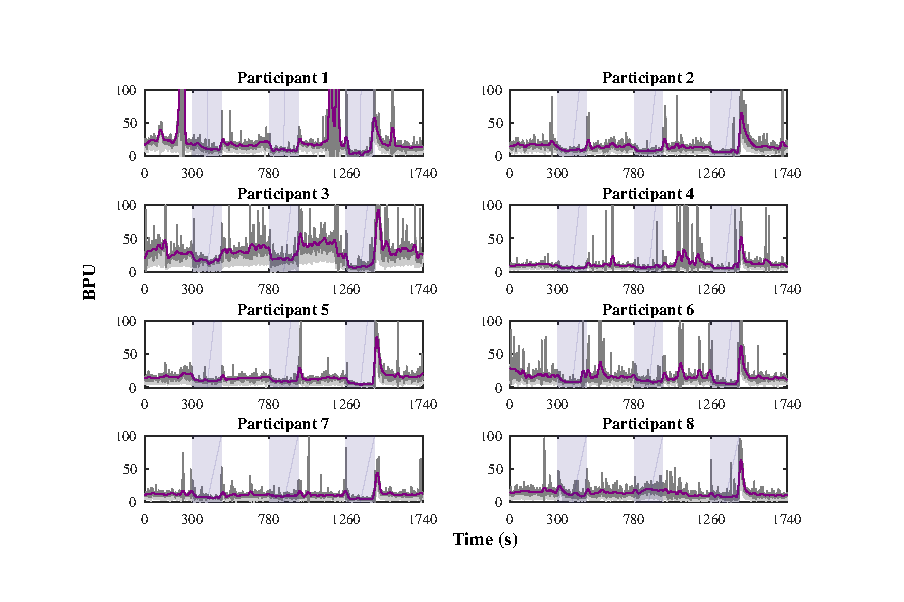
\includegraphics[width=\textwidth,keepaspectratio,trim={1cm 0cm 1.5cm 0cm},clip]{figure_cmp_3}    
	\caption[Results of the LDF in BPU]{Results of the Laser Doppler Flowmetry measurement for all the participants after being converted to BPU. The values presented in purple are equivalent to envelope signal of the peak points.}
	\label{fig:LDF flow}
\end{figure}

Nevertheless, a trend can be noticed in all the participants. During the occlusions a decline in the red blood cell movement can be noticed. It seems that the blockage of the venous return in regions 3 and 5 slowed down the movement of RBC in the capillaries. Additionally, during total occlusion can be appreciated that the amplitude reaches its lower values. After the restitution of the blood flow, the RBC movement depicted a Gaussian bell shape peak in most of the participants. This hyperaemic effect shows an acceleration of the blood cells after the blockage event. This acceleration is evident in every occlusion. Nevertheless, it varies in magnitude with each occlusion. It can be appreciated that the BPU magnitude after the total occlusion is clearly larger on in all participants. In comparison, the other two occlusions created a smaller Gaussian shape response where the one after the partial arterial appears to be slightly larger. Nevertheless, participant 8 seems to be an exception to this rule. The BPU measurements increased slightly during the transition from region 3 to 4. Moreover, contrary to the other participant's waveforms in the transition from partial arterial occlusion to baseline in region 5, his mean BPU decreased. These results obtained from this partaker also could explain some of the adverse readings captured by the iPG signals.

Lastly, during total occlusion, all the mean BPUs of the participants reduced considerably. Then later, when the tourniquet was released, the rush of blood flow can be noticed in the hyperaemic effect registered by the instrument, which was also detected by others instruments. Table \ref{tbl:LDF flow} reviews the values of the mean BPU data obtained. The results displayed there are in complete agreement with the figure previously analysed.

\begin{table}[!htbp]
	\caption{Media perfusion index (flux) calculated form the LDF data for all the regions during the experiment.}
	\label{tbl:LDF flow}
	\centering \small
	\begin{tabular}{p{1.9cm}cccccccc}
		\toprule
		& \textbf{Region 1}
		& \textbf{Region 2}
		& \textbf{Region 3}
		& \textbf{Region 4}
		& \textbf{Region 5}
		& \textbf{Region 6}
		& \textbf{Region 7} \\
		& \textbf{[BPU]}
		& \textbf{[BPU]}
		& \textbf{[BPU]}		
		& \textbf{[BPU]}		
		& \textbf{[BPU]}
		& \textbf{[BPU]}
		& \textbf{[BPU]}\\\midrule
    	Participant 1 & 23.65 & 11.59 & 17.20 &  9.20 & 19.81 & 5.16 & 14.60 \\  
		Participant 2 & 16.88 &  9.10 & 14.44 &  8.19 & 13.17 & 6.07 & 14.83 \\  
		Participant 3 & 29.46 & 17.43 & 32.86 & 19.76 & 41.80 & 7.83 & 33.87 \\  
		Participant 4 &  9.81 &  6.14 &  9.53 &  6.99 & 14.11 & 5.94 & 12.19 \\  
		Participant 5 & 15.56 & 10.35 & 13.85 &  9.28 & 14.02 & 4.73 & 18.03 \\  
		Participant 6 & 18.66 &  8.80 & 16.03 &  9.56 & 15.06 & 6.60 & 14.56 \\  
		Participant 7 & 11.96 &  7.25 & 10.37 &  9.51 & 10.24 & 5.08 & 11.91 \\  
		Participant 8 & 15.54 & 12.40 & 13.85 & 17.93 & 12.29 & 8.40 & 10.97 \\  
		\bottomrule
	\end{tabular}
\end{table}


%%********************************** % Section 9.4 ******************************************
\section{Measurements from the PPG Red-light signal}
\label{section comparison PPG}
The photoplethysmographic device produced information about the change of volume within the vascular bed under the skin. It is capable of detecting either venous or arterial blood change according to the light wavelength used ~\cite{almond1988noninvasive}. The finger probe used all along the experiment contained both, red and infrared sensors. Nevertheless, the red light information was collected because is more sensitive to changes in the venous blood. The device employed in the experiment has an output port which provides the unprocessed raw photoplethysmography waveform. Similarly, as in the iPG signal, the PPG is formed of DC and AC components. The DC portion of the signal is equivalent to the blood volume under the light beam. Moreover, it also contains data about respiratory rate and other physiological information, not required for this experimental setting. On the contrary, the magnitude of the AC component changes synchronously with the cardiac cycle and blood volume under the capillaries. 

The raw signal displayed in \ref{fig:RED PPG} reveals both the DC (on the left) and the AC (on the right) components of all the study participants. Additionally, within the plot, the shaded regions represent each occlusive event during the experiment. The DC component of the signal was obtained by decoding the bottom values that envelope the raw PPG waveform. In other words, the points on the foot of the waveform.  Besides, the AC component of the signal was obtained by subtracting the low envelope of the raw data. Furthermore, the resultant waveform was inverted to leave only the dynamic element of the signal. Last, the peaks detected from the plethysmography waveform were redrawn in black, highlighting the maximum values during all the occlusive events.

\begin{figure}[!htbp]
	\centering
	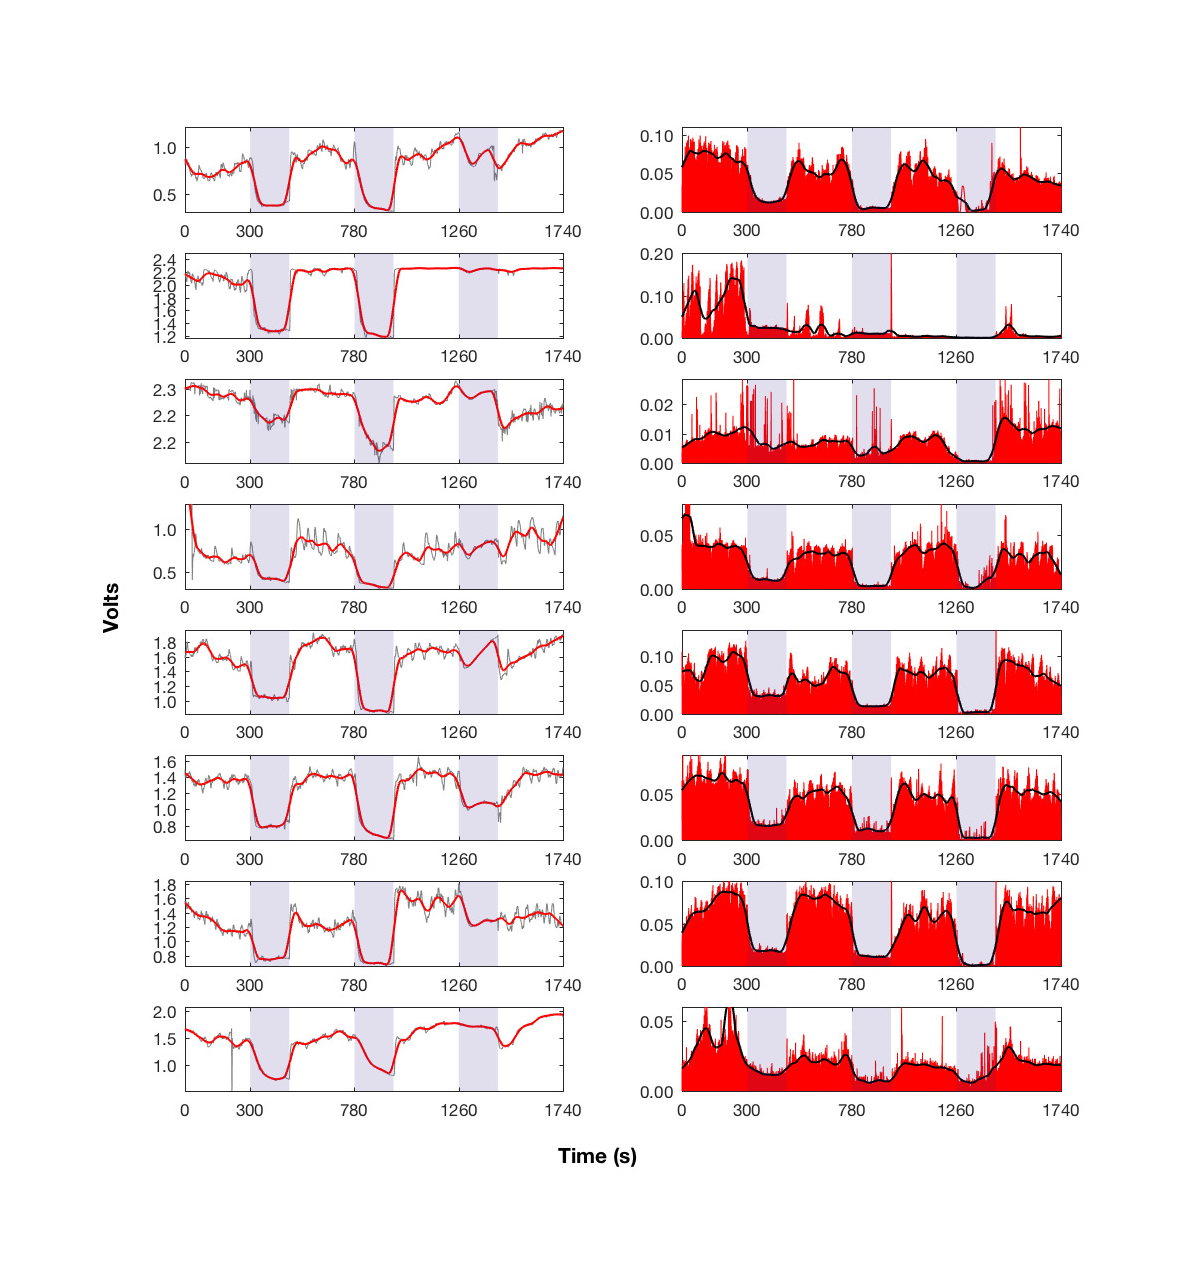
\includegraphics[width=\textwidth,keepaspectratio,trim={1cm 0cm 0cm 0 cm},clip]{figure_cmp_4}
	\centering
	\begin{minipage}[t]{.45\linewidth}
		\centering
		\subcaption{DC component of the PPG waveform for each of the participants}\label{fig:RED PPG AC}
	\end{minipage}%
	\centering
	\begin{minipage}[t]{.45\linewidth}
		\centering
		\subcaption{AC component of the PPG waveform for each of the participants}\label{fig:RED PPG DC}
	\end{minipage}
	\caption[PPG red wavelength measurments, AC and DC components]{PPG measurements using the red spectrum. The plots show the DC and AC components of the waveform. The shaded areas represent the occlusion events during the experiment venous occlusion (region 2), partial arterial occlusion (region 4) and total occlusion (region 6))}
	\label{fig:RED PPG}
\end{figure}

\subsection{Changes in the DC component of the signal}
\label{section comparison 4.1}
Analysing the DC signal can be seen that all the participants showed a definite drop in their DC components during venous occlusion (region 2) and partial arterial occlusion (region 4). The figure portrays that the DC value dropped dramatically in most participants after the occlusive event. Nevertheless, some participants displayed an exponential decrease of their recordings as showed participants 3 and 8 during both occlusive events. 

The visible change of the DC value is confirmed when analysing the mean values of the DC data presented in Table \ref{tbl:PPG RED-DC}. From there, the calculated average baseline before the occlusions were \SI{1.44(055)}{\volt} for Region 1 and \SI{1.51(054)}{\volt} for Region 3.  In contrast, during the occlusive transitions, the DC components dropped about \SI{0.435(0210)}{\milli\volt} and \SI{0.528(0247)}{\milli\volt} for region 2 and region 4 respectively. Comparing the difference in DC values between both events, it can be seen that difference between both is quite small, only \SI{4.47}{\percent}. Nevertheless, during total occlusion, the signals obtained were erratic with no clear shape or direction. Some participants showed a slight decrease, but others did not exhibit significant changes. In general, DC data provided valuable information during the venous and partial arterial occlusion but not conclusive results during total blood flow stoppage. 

\begin{table}[!htbp]
	\caption[Mean peak value of the PPG DC signal for all participants in all regions]{Mean peak value of the PPG DC signal for all the participants in all the regions.}
	\label{tbl:PPG RED-DC}
	\centering \small
	\begin{tabular}{p{1.9cm}cccccccc}
		\toprule
		& \textbf{Region 1}
		& \textbf{Region 2}
		& \textbf{Region 3}
		& \textbf{Region 4}
		& \textbf{Region 5}
		& \textbf{Region 6}
		& \textbf{Region 7} \\
		& \textbf{[\si{\volt}]}
		& \textbf{[\si{\volt}]}
		& \textbf{[\si{\volt}]}		
		& \textbf{[\si{\volt}]}		
		& \textbf{[\si{\volt}]}
		& \textbf{[\si{\volt}]}
		& \textbf{[\si{\volt}]}\\\midrule
		Participant 1 & 0.75 & 0.44 & 0.91 & 0.43 & 0.94 & 0.91 & 1.03 \\  
		Participant 2 & 2.09 & 1.38 & 2.22 & 1.33 & 2.25 & 2.24 & 2.24 \\  
		Participant 3 & 2.24 & 2.20 & 2.24 & 2.16 & 2.23 & 2.24 & 2.20 \\  
		Participant 4 & 0.76 & 0.46 & 0.80 & 0.36 & 0.72 & 0.79 & 0.89 \\  
		Participant 5 & 1.60 & 1.07 & 1.73 & 0.93 & 1.66 & 1.64 & 1.64 \\  
		Participant 6 & 1.36 & 0.84 & 1.38 & 0.76 & 1.41 & 1.08 & 1.35 \\  
		Participant 7 & 1.26 & 0.79 & 1.25 & 0.75 & 1.56 & 1.32 & 1.34 \\  
		Participant 8 & 1.48 & 0.88 & 1.48 & 1.07 & 1.64 & 1.71 & 1.70 \\  
		\bottomrule
	\end{tabular}
\end{table}

\subsection{Changes in the AC component of the signal}
\label{section comparison 4.2}
The AC component also produced a notable swing of magnitude during each blockage event. Compared to the DC, the AC signal not only changed its amplitude all along venous and partial arterial occlusion but also during total occlusion, where reached minimum magnitude which is concurrent with the fact that there is no change of volume at that precise instant. Reviewing the AC signals qualitatively, participant 2, 3 and 5 displayed low-quality waveforms because their amplitudes were quite close to noise levels  (amplitude < \SI{10}{\milli\volt}).   Participant 2 registered noisy waveforms during region 1 of the study and small magnitudes for the rest of the experiment. Besides, participant 3 presented low signal amplitude and over peaks during the whole test, but changes through each occlusion are still visible.

\begin{table}[!htbp]
	\caption[Mean peak value of the PPG AC signal for all participants in all regions]{Mean peak value of the PPG AC signal for all the participants in all the regions.}
	\label{tbl:PPG RED-AC}
	\centering \small
	\begin{tabular}{p{1.9cm}cccccccc}
		\toprule
		& \textbf{Region 1}
		& \textbf{Region 2}
		& \textbf{Region 3}
		& \textbf{Region 4}
		& \textbf{Region 5}
		& \textbf{Region 6}
		& \textbf{Region 7} \\
		& \textbf{[\si{\milli\volt}]}
		& \textbf{[\si{\milli\volt}]}
		& \textbf{[\si{\milli\volt}]}		
		& \textbf{[\si{\milli\volt}]}		
		& \textbf{[\si{\milli\volt}]}
		& \textbf{[\si{\milli\volt}]}
		& \textbf{[\si{\milli\volt}]}\\\midrule
		Participant 1 & 724.83 & 180.45 & 546.76 &  66.13 & 490.87 & 109.85 & 441.54   \\  
		Participant 2 & 926.02 & 245.24 & 158.34 & 110.32 &  51.30 &   5.97 &  92.58   \\  
		Participant 3 &  94.21 &  69.72 &  68.76 &  37.19 &  71.62 &  10.54 & 122.67   \\  
		Participant 4 & 436.74 &  92.42 & 315.26 &  37.22 & 354.44 &  58.08 & 296.36   \\  
		Participant 5 & 873.38 & 324.60 & 638.53 & 155.21 & 703.81 &  51.36 & 751.62   \\  
		Participant 6 & 658.05 & 188.75 & 501.10 & 112.57 & 480.41 &  38.14 & 517.01   \\  
		Participant 7 & 731.50 & 190.43 & 746.34 & 125.76 & 547.89 &  26.92 & 660.43   \\  
		Participant 8 & 360.69 & 130.06 & 216.80 &  74.43 & 168.52 &  89.77 & 217.06   \\ 
		\bottomrule
	\end{tabular}
\end{table}

From the numeric point of view, Table \ref{tbl:PPG RED-AC} shows the average values of the amplitude in \si{\milli\volt}. During all the baseline measurements (regions 1,3,5 and 7), the mean peak value was \SI{436.41(11081)}{\milli\volt}. However, it can be notices the overshooting during region which displayed values considerably higher than the mean.  

In general, during venous occlusion, the signal amplitude decreased in all the experiment members in about \SI{422.97(21217)}{\milli\volt}. However, participant 3 was an outlier showing the smallest change (\SI{24.50}{\milli\volt}) compared to the rest of the signals; it seems that the poor quality signal affected the whole measurement. After the cuff's pressure had been released during the transition from venous occlusion to baseline, participants 2 and 3 showed a decrease of their mean amplitude, again the poor signal quality of these two study members showed inconclusive measurements. The rest of the partakers displayed a recovery in their signal peak to a peak of approximately \SI{221.28(21124)}{\milli\volt}. 

During partial arterial occlusion in region 4, the physiological response was detected by the device. In this case, all participants registered a decrease in their mean PPG signals amplitude of an average of \SI{309.14(21943)}{\milli\volt}. When comparing mean values during occlusions in region 2 and 4, the signal amplitude in region 4 was slightly lower than the one in region 2 by about \SI{87.86(4691)}{\milli\volt}, the difference between both circulatory occlusions \SI{49.75}{\percent}.

Finally, throughout total occlusion, also all the participants exhibited a substantial decrease in their AC amplitudes as expected because of the absence of blood flow in the vessels. All in all, signals went below \SI{109}{\milli\volt} with an average value of \SI{48.83(3662)}{\milli\volt}. In fact, this confirms that the measurements from participants 3 were below this level. 

In conclusion, the PPG waveform experienced changes of DC and AC components during all the occlusions throughout the study. The DC signal was able to detect changes during venous and partial arterial occlusions. The difference of their mean DC values of these two events was minimal, only \SI{4.47}{\percent}. Furthermore, during total occlusion, there was not any noticeable change in DC value of the signal.  On the other hand, the AC component was able to distinguish between venous and partial occlusion. Indeed, the difference between these two regions was nearly \SI{50}{\percent}. Moreover, the signal lost most of its magnitude during total occlusion due to the lack of blood flow.

%%********************************** % Section 9.5 ******************************************
\section{Conclusion}
\label{section comparison 5}
This chapter presented the general changes of the waveforms during the whole experiment. All the instruments exhibited a different response according to the technology used by each one. The data obtained from the impedance device was converted to blood flow to understand the changes in venous circulation. The Doppler Ultrasound method showed changes in the arterial circulation while the optical techniques presented alterations in the microcirculation. 

Converting the impedance APA waveform into blood flow using the Nyboer equation \ref{eq:nyober dV}, as found in the literature found in the literature \cite{corciova2011peripheral, porter1985measurement, brown1975impedance, marks1985computer}, reflected a rise in the blood rate. The increase in the measurement was expected entirely as the flow rate is directly proportional to the amplitude of the impedance. As presented in chapter \ref{chapter apa}, the APA waveform depicted an increment of its systolic peak during venous and partial arterial occlusions. For instance, during venous occlusion in region 2, the blood rate increased of about \SI{33}{\percent} compared to the previous baseline in region 1. It seems that the rise of blood flow might be related to a vasodilation response where the cross-sectional area of the veins in the forearm enlarged allowing the blood pooling. 

However, comparing venous and partial arterial occlusions showed a different result regarding the increase in blood flow. Although both showed a rise in their waveform systolic peaks, the calculated flow rate during partial occlusion was in average \SI{8.4}{\percent} in region 4. One might expect the blood flow to lessen as the normal artery flow is restricted. Nevertheless, the impedimetric measurement presented a slight increase in blood flow. It seems that once again the rise in the calculated blood flow might be related to vasodilation during the occlusion. The extra blood flow coming into the expanded vein might be seen as a rush in the blood rate.

The Doppler Ultrasound method detected changes in the arterial flow. The sensor of the instrument was pointing towards the radial artery providing information about the changes of arterial inflow within the forearm. Some of the drawbacks of this approach are that taking proper measurements require a person with specific skills to target the vessel under study accurately, such as steady-hand and acute hearing, on top of that, keeping a fixed angle of measurements for prolonged periods of time can be challenging for any person. Some of these issues were addressed during the experiment by using a fix lab clamp, but still, any movement from the participant would misalign the sensor producing errors in the data recorded. In general, the instrument detected changes in arterial flow during partial arterial and total occlusion. The arterial blood rate reduced to about \SI{48.79(1191)}{\percent} during partial arterial occlusion and practically zero during complete obstruction.

In comparison, the optical methods provided data about the venous circulation. The PPG in the red spectrum correlated to the venous circulation whereas LDF offered details of the blood cells moving in the capillary bed. One of the weaknesses of the optical methods is that the measurement is limited to a small confined volume, where is hard to estimate the depth which the light beam is travelling into the tissue accurately. However, optical methods do not require the use of a specialist to take measurements making it appropriate for an unsupervised operation.



%********************************** %Nomenclature found  *************************************
\nomenclature[z-PTT]{PTT}{Pulse transit time}